\chapter{Complejación}\label{ch:b1:complexation}

Viértase un poco de disolución de amoniaco en sulfato de cobre(II), de
color azul pálido: se forma enseguida un precipitado azul pálido. Viértase
más, y el precipitado se disuelve en una disolución de un azul intenso,
casi de tinta. Nada en los capítulos de ácido--base o de precipitación
explica el segundo paso. Las moléculas de amoniaco se han unido al ion
cobre mediante sus \omterm{def:b1:lewis-resonance-vsepr:lewis}{pares no enlazantes} y han formado una especie nueva,
un \omterm{def:b1:complexation:complex}{complejo}, más estable que el hidróxido y de otro color. Los \omterm{def:b1:complexation:complex}{complejos}
transportan el oxígeno en la sangre, retienen el metal en la clorofila y
en la vitamina B$_{12}$, ablandan el agua dura y disuelven metales que
nada más disuelve. Este capítulo los trata como un intercambio más de
partículas en el agua, con sus propias constantes y sus propios
diagramas.

\begin{recall}
Los \omterm{def:b1:lewis-resonance-vsepr:lewis-acid}{ácidos de Lewis} (aceptores de pares de electrones), las \omterm{def:b1:lewis-resonance-vsepr:lewis-acid}{bases de Lewis}
(dadores de pares de electrones) y el \omterm{def:b1:lewis-resonance-vsepr:lewis-acid}{enlace dativo} se definieron en el
\cref{ch:b1:lewis-resonance-vsepr}. Los \omterm{def:b1:predominant-reaction:predominance}{diagramas de predominio} y el
método de la \omterm{def:b1:predominant-reaction:predominant-reaction}{reacción predominante} proceden del
\cref{ch:b1:predominant-reaction}; el \omterm{def:b1:precipitation:solubility-product}{producto de solubilidad} y la
condición de precipitación, del \cref{ch:b1:precipitation}.
\end{recall}

\begin{omfigure}
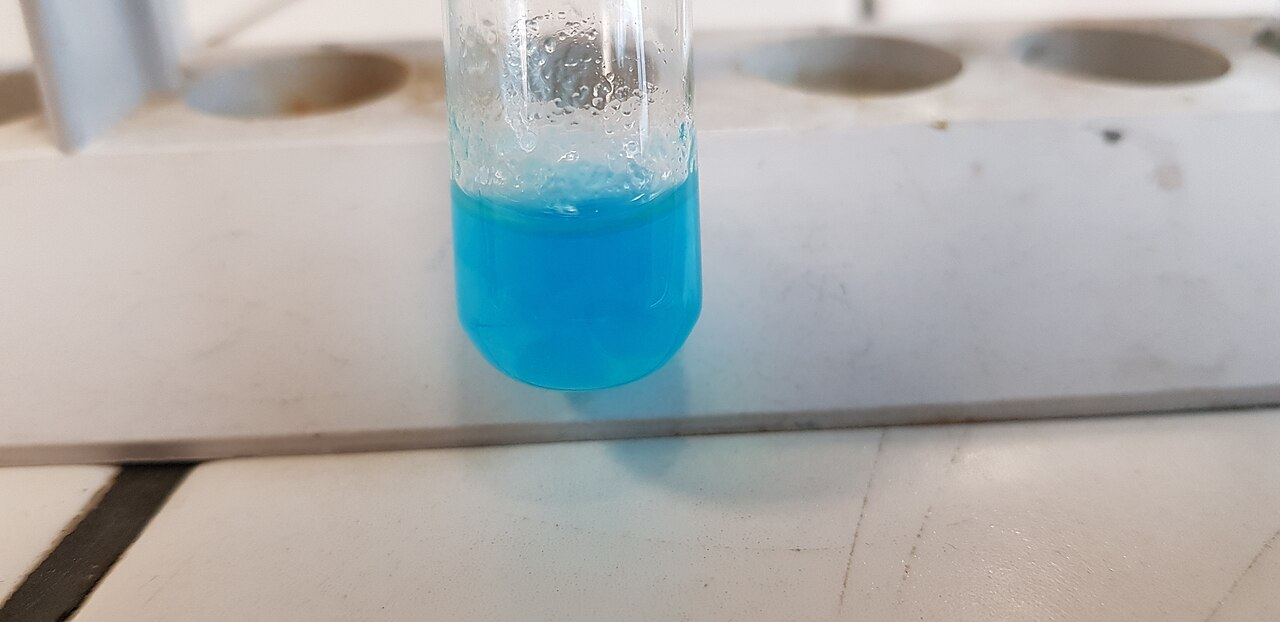
\includegraphics[height=4.2cm]{images/book2/copper-hydroxide.jpg}\hspace{0.6em}%
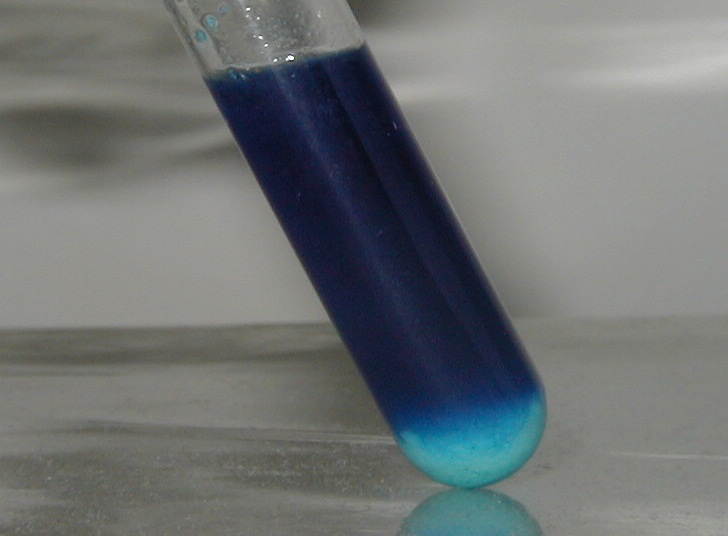
\includegraphics[height=4.2cm]{images/book2/copper-ammine.jpg}

{\small A la izquierda, una suspensión de hidróxido de cobre(II), azul
pálido (fotografía de Alvy16, CC BY 4.0). A la derecha, con más amoniaco
el sólido se disuelve dando el ion tetraamincobre(II), de un azul
intenso; en el fondo del tubo queda algo de hidróxido sin disolver
(fotografía de Chemicalinterest, dominio público). Ambas de Wikimedia
Commons.}
\end{omfigure}

\section{Complejos y ligandos}

\begin{definition}[Complejo, átomo central, ligando]\label{def:b1:complexation:complex}
Un \emph{complejo}\index{complejo} es una especie formada por un
\emph{átomo central}\index{atomo central@átomo central} o ion central,
normalmente un catión metálico que actúa como \omterm{def:b1:lewis-resonance-vsepr:lewis-acid}{ácido de Lewis}, unido por
\omterm{def:b1:lewis-resonance-vsepr:lewis-acid}{enlaces dativos} a moléculas o iones que actúan como \omterm{def:b1:lewis-resonance-vsepr:lewis-acid}{bases de Lewis}, los
\emph{ligandos}\index{ligando}. Su fórmula se escribe entre corchetes, con
su carga total: $[\ce{Cu(NH3)4}]^{2+}$,
$[\ce{Fe(CN)6}]^{4-}$, $[\ce{Ag(NH3)2}]^{+}$, $[\ce{FeSCN}]^{2+}$.
\end{definition}

La carga del \omterm{def:b1:complexation:complex}{complejo} es la suma de las cargas del ion central y de los
\omterm{def:b1:complexation:complex}{ligandos}: $\mathrm{Fe^{2+}}$ y seis \ce{CN-} dan
$[\ce{Fe(CN)6}]^{4-}$. Un \omterm{def:b1:complexation:complex}{ligando} necesita al menos un \omterm{def:b1:lewis-resonance-vsepr:lewis}{par no enlazante}:
\ce{NH3}, \ce{H2O}, \ce{OH-}, \ce{Cl-}, \ce{CN-}, \ce{SCN-} (unido por S o
por N). Todo ion metálico en el agua es de hecho ya un \omterm{def:b1:complexation:complex}{complejo} con
moléculas de agua como \omterm{def:b1:complexation:complex}{ligandos}, $[\ce{Cu(H2O)6}]^{2+}$ o
$[\ce{Fe(H2O)6}]^{3+}$; formar otro \omterm{def:b1:complexation:complex}{complejo} significa intercambiar esas
moléculas de agua por otros \omterm{def:b1:complexation:complex}{ligandos}, y los \omterm{def:b1:complexation:complex}{ligandos} agua se omiten en las
fórmulas, igual que se escribe \ce{H3O+} para el protón hidratado.

\begin{omfigure}
\begin{tikzpicture}[font=\small, line cap=round]
  % [Ag(NH3)2]+ : linear
  \begin{scope}
    \node (ag) at (0,0) {\ce{Ag}};
    \node (n1) at (-1.2,0) {\ce{H3N}};
    \node (n2) at (1.2,0) {\ce{NH3}};
    \draw[thick] (n1) -- (ag) -- (n2);
    \node at (0,-1.75) {$[\ce{Ag(NH3)2}]^{+}$, lineal};
  \end{scope}
  % [Cu(NH3)4]2+ : square plane in perspective
  \begin{scope}[xshift=4.3cm, every node/.style={fill=white, inner sep=1.5pt}]
    \node (cu) at (0,0) {\ce{Cu}};
    \node (a) at (-1.45,-0.5) {\ce{H3N}};
    \node (b) at (1.45,0.5) {\ce{NH3}};
    \node (c) at (0.85,-0.9) {\ce{NH3}};
    \node (d) at (-0.85,0.9) {\ce{H3N}};
    \begin{pgfonlayer}{background}
    \draw[gray, dashed] (a.center) -- (c.center) -- (b.center) -- (d.center) -- cycle;
    \end{pgfonlayer}
    \draw[thick] (cu) -- (a); \draw[thick] (cu) -- (b);
    \draw[thick] (cu) -- (c); \draw[thick] (cu) -- (d);
    \node at (0,-1.75) {$[\ce{Cu(NH3)4}]^{2+}$, plano-cuadrado};
  \end{scope}
  % [Fe(CN)6]4- : octahedron
  \begin{scope}[xshift=9.2cm, every node/.style={fill=white, inner sep=1.5pt}]
    \node (fe) at (0,0) {\ce{Fe}};
    \node (t) at (0,1.3) {\ce{CN}};
    \node (u) at (0,-1.3) {\ce{CN}};
    \node (l) at (-1.45,-0.45) {\ce{NC}};
    \node (r) at (1.45,0.45) {\ce{CN}};
    \node (f) at (0.8,-0.8) {\ce{CN}};
    \node (k) at (-0.8,0.8) {\ce{NC}};
    \begin{pgfonlayer}{background}
    \draw[gray, dashed] (l.center) -- (f.center) -- (r.center) -- (k.center) -- cycle;
    \end{pgfonlayer}
    \foreach \x in {t,u,l,r,f,k} \draw[thick] (fe) -- (\x);
    \node at (0,-1.75) {$[\ce{Fe(CN)6}]^{4-}$, octaédrico};
  \end{scope}
\end{tikzpicture}

{\small Tres \omterm{def:b1:complexation:complex}{complejos} y sus formas. Cada trazo es un \omterm{def:b1:lewis-resonance-vsepr:lewis-acid}{enlace dativo} desde
el \omterm{def:b1:lewis-resonance-vsepr:lewis}{par no enlazante} del \omterm{def:b1:complexation:complex}{ligando} (el N del amoniaco, el C del cianuro)
hasta el ion metálico; las líneas discontinuas delimitan el cuadrado de
cuatro \omterm{def:b1:complexation:complex}{ligandos}. Las formas de los \omterm{def:b1:complexation:complex}{complejos} se explican en el volumen
del segundo año.}
\end{omfigure}

\begin{definition}[Ligando polidentado, quelato]\label{def:b1:complexation:chelate}
Un \omterm{def:b1:complexation:complex}{ligando} que se une al mismo ion central a través de varios de sus
átomos a la vez es un \emph{ligando polidentado}\index{ligando polidentado};
el \omterm{def:b1:complexation:complex}{complejo} que forma, en el que el \omterm{def:b1:complexation:complex}{ligando} cierra anillos alrededor del
ion metálico, es un \emph{quelato}\index{quelato}. La etilendiamina
\ce{H2N-CH2-CH2-NH2} se une por dos átomos de N; el ion oxalato
\ce{C2O4^2-}, por dos átomos de O, y el ion etilendiaminotetraacetato
(\emph{EDTA}, que se escribe \ce{Y^4-}), por dos átomos de N y cuatro de
O.
\end{definition}

\begin{omfigure}
\setchemfig{atom sep=1.9em}
\chemfig{N(-[3]-[2]C(=[1]O)-[3]O^{-})(-[5]-[6]C(=[7]O)-[5]O^{-})-[0]-[0]N(-[1]-[2]C(=[3]O)-[1]O^{-})(-[7]-[6]C(=[5]O)-[7]O^{-})}
\hspace{2.2em}
\begin{tikzpicture}[font=\small, baseline=(ca.base)]
  \node[circle, draw, thick, fill=omDef!12, inner sep=1.5pt] (ca) at (0,0) {\ce{Ca}};
  \node (n1) at (-1.15,-0.35) {N};
  \node (n2) at (0.55,-0.6) {N};
  \node (o1) at (0,1.35) {O};
  \node (o2) at (0,-1.35) {O};
  \node (o3) at (1.15,0.35) {O};
  \node (o4) at (-0.55,0.6) {O};
  \foreach \x in {n1,n2,o1,o2,o3,o4} \draw[thick, omDef] (ca) -- (\x);
  \draw[omProp, thick] (n1) .. controls (-0.57,-0.95) .. (n2);
  \draw[omProp, thick] (n1) .. controls (-1.05,0.95) .. (o1);
  \draw[omProp, thick] (n1) .. controls (-1.5,0.25) .. (o4);
  \draw[omProp, thick] (n2) .. controls (0.5,-1.6) .. (o2);
  \draw[omProp, thick] (n2) .. controls (1.5,-0.3) .. (o3);
\end{tikzpicture}

{\small A la izquierda, el ion EDTA, \ce{Y^4-}, con sus dos átomos de N y
sus cuatro grupos carboxilato. A la derecha, el \omterm{def:b1:complexation:chelate}{quelato} calcio--EDTA
$[\ce{CaY}]^{2-}$, de forma esquemática: los seis átomos dadores (enlaces
azules) ocupan los vértices de un octaedro alrededor del ion, con los dos
átomos de N contiguos, y las cadenas carbonadas del \omterm{def:b1:complexation:complex}{ligando} (en naranja)
cierran cinco anillos de cinco átomos cada uno, los anillos \omterm{def:b1:complexation:chelate}{quelato}.}
\end{omfigure}

El ion EDTA retiene un ion calcio con firmeza suficiente para ser el
reactivo de la valoración de la dureza del agua
(\cref{ch:b1:titration-methods}).

\section{Constantes de formación y de disociación}

\begin{definition}[Constantes de formación y de disociación]\label{def:b1:complexation:formation-constant}
Para un ion central M y un \omterm{def:b1:complexation:complex}{ligando} L (se omiten las cargas), la
\emph{constante de formación global}\index{constante de formacion global@constante de formación global} de
$\mathrm{ML}_n$ es la constante $\beta_n$ de
$\mathrm{M} + n\,\mathrm{L} \rightleftharpoons \mathrm{ML}_n$,
\[
  \beta_n = \frac{[\mathrm{ML}_n]}{[\mathrm{M}][\mathrm{L}]^n} .
\]
La \emph{constante de formación sucesiva}\index{constante de formacion sucesiva@constante de formación sucesiva}
$K_i$ es la de la adición de un \omterm{def:b1:complexation:complex}{ligando},
$\mathrm{ML}_{i-1} + \mathrm{L} \rightleftharpoons \mathrm{ML}_i$. La
\emph{constante de disociación}\index{constante de disociacion@constante de disociación} es la
inversa, $K_d = 1/K_i$, y $\mathrm{p}K_d = \log K_i$, de modo que un par
\omterm{def:b1:complexation:complex}{complejo}/\omterm{def:b1:complexation:complex}{ligando} se describe exactamente como un \omterm{def:b1:predominant-reaction:bronsted}{par ácido--base}, con el
\omterm{def:b1:complexation:complex}{ligando} en lugar del protón.
\end{definition}

\begin{proposition}[Constantes globales y sucesivas]\label{prop:b1:complexation:beta-k}
$\beta_n = K_1 K_2 \cdots K_n$, es decir,
$\log\beta_n = \sum_{i=1}^n \log K_i$ y $\log K_i = \log\beta_i -
\log\beta_{i-1}$ (con $\beta_0 = 1$).
\end{proposition}

\begin{proof}
La formación de $\mathrm{ML}_n$ a partir de M es la suma de las $n$
adiciones sucesivas; la constante de una suma de reacciones es el
producto de sus constantes (\cref{ch:b1:extent-q-and-k}). Directamente:
$K_1 K_2\cdots K_n = \frac{[\mathrm{ML}]}{[\mathrm{M}][\mathrm{L}]}
\frac{[\mathrm{ML_2}]}{[\mathrm{ML}][\mathrm{L}]}\cdots
\frac{[\mathrm{ML}_n]}{[\mathrm{ML}_{n-1}][\mathrm{L}]}$, y las
concentraciones intermedias se simplifican.
\end{proof}

\begin{omfigure}
\begin{tabular}{lll}
\hline
\omterm{def:b1:complexation:complex}{complejo} & $\log\beta_n$ & $\log K_i$ \\
\hline
$[\ce{Cu(NH3)_n}]^{2+}$, de $n = 1$ a 4 & 4.10, 7.51, 10.33, 12.36 & 4.10, 3.41, 2.82, 2.03 \\
$[\ce{Ag(NH3)_n}]^{+}$, $n = 1, 2$ & 3.32, 7.22 & 3.32, 3.90 \\
$[\ce{Zn(OH)4}]^{2-}$ & $\log\beta_4 = 14.45$ & \\
$[\ce{FeSCN}]^{2+}$, $[\ce{FeF}]^{2+}$ & 2.96; 6.85 & \\
$[\ce{CaY}]^{2-}$, $[\ce{MgY}]^{2-}$, $[\ce{NiY}]^{2-}$ & 12.69, 10.90, 20.54 & \\
\hline
\end{tabular}

\smallskip
{\small Constantes de formación a \qty{25}{\celsius}. Las constantes de
los \omterm{def:b1:complexation:complex}{complejos} amoniacales, hidroxo, tiocianato y fluoro se calculan a
partir de entalpías libres estándar de formación tabuladas; las
constantes del EDTA son valores seleccionados críticamente a fuerza
iónica nula, como los $\mathrm{p}K_a$ del EDTA que se usan más abajo,
2.23, 3.15, 6.80 y 11.24.}
% ledger: dfg:Cu2+_ao, dfg:CuNH32+_ao, dfg:Cu_NH322+_ao, dfg:Cu_NH332+_ao, dfg:Cu_NH342+_ao, dfg:NH3_ao (computed in figdata/bachelor-1/aqueous-constants.py)
% ledger: dfg:Ag+_ao, dfg:AgNH3+_ao, dfg:Ag_NH32+_ao, dfg:Fe3+_ao, dfg:SCN-_ao, dfg:FeSCN2+_ao, dfg:F-_ao, dfg:FeF2+_ao (computed, same script)
% ledger: logb:Ca-edta, logb:Mg-edta, logb:Ni-edta, pka:edta1, pka:edta2, pka:edta3, pka:edta4
\end{omfigure}

Las constantes sucesivas de los \omterm{def:b1:complexation:complex}{complejos} amoniacales del cobre
disminuyen, $K_1 > K_2 > K_3
> K_4$: cada molécula de amoniaco añadida deja menos posiciones libres y
hace al \omterm{def:b1:complexation:complex}{complejo} algo menos ávido de la siguiente. Es el orden habitual.
La plata es una excepción: $K_2 > K_1$, con consecuencias que se extraen
en el problema de fin de semana.

\section{Predominio en pL}

\begin{definition}[Escala de pL]\label{def:b1:complexation:pl-diagram}
Para un \omterm{def:b1:complexation:complex}{ligando} L, $\mathrm{pL} = -\log[\mathrm{L}]$, donde $[\mathrm{L}]$
es la concentración del \omterm{def:b1:complexation:complex}{ligando} libre. Una \emph{escala de pL}\index{escala de pL}
es un eje de pL sobre el que se dibujan los dominios de predominio del
ion central y de sus \omterm{def:b1:complexation:complex}{complejos}, igual que se dibujan los dominios de los
ácidos y las bases sobre un eje de pH.
\end{definition}

\begin{proposition}[Fronteras en pL]\label{prop:b1:complexation:pl-boundaries}
Para el par $\mathrm{ML}_i/\mathrm{ML}_{i-1}$,
\[
  \mathrm{pL} = \log K_i + \log\frac{[\mathrm{ML}_{i-1}]}{[\mathrm{ML}_i]} ,
\]
de modo que $\mathrm{ML}_{i-1}$ predomina para $\mathrm{pL} > \log K_i$, y
$\mathrm{ML}_i$, para $\mathrm{pL} < \log K_i$. Cuando los $\log K_i$
disminuyen con $i$, el diagrama es una sucesión de dominios:
$\mathrm{ML}_n$ a pL pequeño (mucho \omterm{def:b1:complexation:complex}{ligando}), después
$\mathrm{ML}_{n-1}$, y así hasta M a pL grande.
\end{proposition}

\begin{proof}
Se toma el logaritmo de $K_i = [\mathrm{ML}_i]/([\mathrm{ML}_{i-1}][\mathrm{L}])$:
$\log K_i = \log\frac{[\mathrm{ML}_i]}{[\mathrm{ML}_{i-1}]} + \mathrm{pL}$.
Las dos formas son iguales en $\mathrm{pL} = \log K_i$, y el cociente
cambia en un factor diez por unidad de pL. El dominio de $\mathrm{ML}_i$
está entre $\log K_{i+1}$ y $\log K_i$, y solo existe si $\log K_{i+1} < \log
K_i$.
\end{proof}

\begin{method}[Trazar un diagrama en pL]\label{met:b1:complexation:pl-diagram}
\begin{enumerate}
  \item A partir de los $\log\beta_n$, se calculan los $\log K_i$
        sucesivos.
  \item Si disminuyen, se coloca cada uno en su frontera sobre el eje de
        pL: el \omterm{def:b1:complexation:complex}{complejo} con más \omterm{def:b1:complexation:complex}{ligandos} a la izquierda (pL pequeño) y el
        ion libre a la derecha.
  \item Si algún $\log K_{i+1} > \log K_i$, el \omterm{def:b1:complexation:complex}{complejo} $\mathrm{ML}_i$ no
        tiene dominio: reacciona consigo mismo dando $\mathrm{ML}_{i-1}$ y
        $\mathrm{ML}_{i+1}$. Se suprime y se traza una sola frontera
        entre $\mathrm{ML}_{i-1}$ y $\mathrm{ML}_{i+1}$ en
        $\frac12(\log K_i + \log K_{i+1})$.
\end{enumerate}
\end{method}

\begin{omfigure}
\begin{tikzpicture}
\begin{axis}[
  width=0.78\linewidth, height=5.2cm, xmin=0, xmax=7, ymin=0, ymax=1.05,
  axis x line=bottom, axis y line=left, xlabel={$\mathrm{pNH_3}$},
  ylabel={fracción de cobre},
  tick label style={font=\small}, label style={font=\small}]
\addplot[omThm, thick] table[x=pL, y=M] {figdata/out/bachelor-1-ammine-distribution-copper.dat};
\addplot[omProp, thick] table[x=pL, y=ML] {figdata/out/bachelor-1-ammine-distribution-copper.dat};
\addplot[omMeth, thick] table[x=pL, y=ML2] {figdata/out/bachelor-1-ammine-distribution-copper.dat};
\addplot[black!60, thick] table[x=pL, y=ML3] {figdata/out/bachelor-1-ammine-distribution-copper.dat};
\addplot[omDef, very thick] table[x=pL, y=ML4] {figdata/out/bachelor-1-ammine-distribution-copper.dat};
\node[omDef, font=\small, anchor=west] at (axis cs:0.15,0.78) {$n = 4$};
\node[black!60, font=\small] at (axis cs:2.42,0.63) {3};
\node[omMeth, font=\small] at (axis cs:3.12,0.55) {2};
\node[omProp, font=\small] at (axis cs:3.76,0.58) {1};
\node[omThm, font=\small, anchor=east] at (axis cs:6.9,0.84) {\ce{Cu^2+}};
\end{axis}
\end{tikzpicture}

\begin{tikzpicture}[font=\small, x=1.25cm]
  \draw[->, thick] (0,0) -- (7.2,0) node[right] {$\mathrm{pNH_3}$};
  \foreach \x/\l in {2.03/2.03, 2.82/2.82, 3.41/3.41, 4.10/4.10}
    \draw (\x,0.12) -- (\x,-0.12) node[below] {\l};
  \node[above] at (1.0,0.08) {$[\ce{Cu(NH3)4}]^{2+}$};
  \node[above, font=\scriptsize] at (2.42,0.08) {3};
  \node[above, font=\scriptsize] at (3.12,0.08) {2};
  \node[above, font=\scriptsize] at (3.76,0.08) {1};
  \node[above] at (5.6,0.08) {\ce{Cu^2+}};
  \begin{scope}[yshift=-1.25cm]
  \draw[->, thick] (0,0) -- (7.2,0) node[right] {$\mathrm{pNH_3}$};
  \draw (3.61,0.12) -- (3.61,-0.12) node[below] {3.61};
  \draw[dotted] (3.32,0.3) -- (3.32,-0.1); \draw[dotted] (3.90,0.3) -- (3.90,-0.1);
  \node[above] at (1.6,0.08) {$[\ce{Ag(NH3)2}]^{+}$};
  \node[above] at (5.4,0.08) {\ce{Ag+}};
  \end{scope}
\end{tikzpicture}

{\small Arriba, fracciones del cobre(II) presente como \ce{Cu^2+} y como
$[\ce{Cu(NH3)_n}]^{2+}$ (de $n = 1$ a 4) en función de $\mathrm{pNH_3}$.
En el centro, el \omterm{def:b1:predominant-reaction:predominance}{diagrama de predominio} de los \omterm{def:b1:complexation:complex}{complejos} amoniacales del
cobre, con las fronteras en los $\log K_i$. Abajo, la plata, donde
$\log K_2 = 3.90 > \log K_1 = 3.32$ (punteado): $[\ce{AgNH3}]^{+}$ no
tiene dominio, y hay una sola frontera en
$\frac12\log\beta_2 = 3.61$.}
\end{omfigure}

\begin{example}[El cobre en amoniaco de \texorpdfstring{\qty{0.010}{mol/L}}{0.010 mol/L}]\label{ex:b1:complexation:cu}
Con $[\ce{NH3}] = \qty{0.010}{mol/L}$ libre, $\mathrm{pNH_3} = 2.0$ está
en el dominio de $[\ce{Cu(NH3)3}]^{2+}$, pero cerca de la frontera 2.03
con $[\ce{Cu(NH3)4}]^{2+}$: ambos están casi en la misma proporción. Las
fracciones son proporcionales a $\beta_n[\ce{NH3}]^n = 10^{\log\beta_n - 2n}$,
es decir,
$1 : 10^{2.10} : 10^{3.51} : 10^{4.33} : 10^{4.36}$, de modo que hay un
\qty{48}{\percent} de $[\ce{Cu(NH3)4}]^{2+}$, un \qty{45}{\percent} de
$[\ce{Cu(NH3)3}]^{2+}$, un \qty{7}{\percent} de $[\ce{Cu(NH3)2}]^{2+}$ y
casi nada de \ce{Cu^2+} libre.
\end{example}

\section{Competencias}

Un \omterm{def:b1:complexation:complex}{ligando} puede ser reclamado por dos iones metálicos, y un ion
metálico, por dos \omterm{def:b1:complexation:complex}{ligandos}, y ambos participan además en equilibrios de
precipitación y ácido--base. Cada competencia es una reacción más, cuya
constante combina las constantes ya conocidas; el método de la \omterm{def:b1:predominant-reaction:predominant-reaction}{reacción
predominante} del \cref{ch:b1:predominant-reaction} se aplica entonces
sin cambios.

\begin{example}[Dos ligandos para el hierro(III)]\label{ex:b1:complexation:scn-f}
Una gota de tiocianato en una disolución de hierro(III) da el
$[\ce{FeSCN}]^{2+}$, rojo sangre; los iones fluoruro lo decoloran:
\[
  [\ce{FeSCN}]^{2+} + \ce{F-} \rightleftharpoons [\ce{FeF}]^{2+} + \ce{SCN-},
  \qquad K = \frac{\beta(\ce{FeF})}{\beta(\ce{FeSCN})} = 10^{6.85 - 2.96} =
  10^{3.89} .
\]
El \omterm{def:b1:complexation:complex}{complejo} más fuerte (de mayor $\beta$) se queda con el ion metálico,
exactamente como el ácido más fuerte cede su protón a la base más fuerte.
\end{example}

\begin{proposition}[Complejación frente a precipitación]\label{prop:b1:complexation:competition-precipitation}
Un sólido MX se disuelve en un \omterm{def:b1:complexation:complex}{ligando} L según
$\mathrm{MX(s)} + n\,\mathrm{L} \rightleftharpoons \mathrm{ML}_n + \mathrm{X}$,
de constante $K = \beta_n K_s$. Si el \omterm{def:b1:complexation:complex}{complejo} es la única forma de M en
disolución y la concentración de \omterm{def:b1:complexation:complex}{ligando} libre es $[\mathrm{L}]$, la
\omterm{def:b1:precipitation:solubility}{solubilidad} es $s = \sqrt{K}\,[\mathrm{L}]^{n/2}$.
\end{proposition}

\begin{proof}
La reacción es la suma de la disolución (constante $K_s$) y de la
formación de $\mathrm{ML}_n$ ($\beta_n$). En la saturación, $[\mathrm{ML}_n]
= [\mathrm{X}] = s$ y $K = s^2/[\mathrm{L}]^n$.
\end{proof}

\begin{method}[Disolver un precipitado por complejación]\label{met:b1:complexation:dissolve-precipitate}
\begin{enumerate}
  \item Se escribe la reacción de disolución que da el \omterm{def:b1:complexation:complex}{complejo} y se
        calcula
        $K = \beta_n K_s$.
  \item Si $K$ es grande, la disolución es \omterm{def:b1:extent-q-and-k:quantitative}{cuantitativa} mientras haya
        \omterm{def:b1:complexation:complex}{ligando} suficiente; si es pequeña, se calcula la concentración de
        \omterm{def:b1:complexation:complex}{ligando} libre necesaria para que se disuelva la cantidad de
        sólido:
        $[\mathrm{L}]^n = s^2/K$.
  \item Se suma el \omterm{def:b1:complexation:complex}{ligando} unido en el \omterm{def:b1:complexation:complex}{complejo}, $n s$, para obtener el
        \omterm{def:b1:complexation:complex}{ligando} total que hay que introducir.
  \item Se comprueba que el ion metálico libre es despreciable:
        $[\mathrm{M}] = K_s/s
        \ll s$.
\end{enumerate}
\end{method}

Con amoniaco, el cloruro de plata ($K = 10^{7.22 - 9.75} = 10^{-2.53}$)
se disuelve en disolución moderadamente concentrada, mientras que el
yoduro de plata ($K = 10^{-8.85}$) no: el problema de fin de semana lo
aprovecha para distinguir los haluros.

\begin{proposition}[Complejación frente a acidez]\label{prop:b1:complexation:ligand-acidity}
Si el \omterm{def:b1:complexation:complex}{ligando} es una base $\mathrm{L}$ de un ácido $\mathrm{HL}$ (y
eventualmente de formas más protonadas), solo está disponible la fracción
$[\mathrm{L}]/c_L =
1/\alpha$ del \omterm{def:b1:complexation:complex}{ligando} no unido al metal, con
\[
  \alpha = 1 + \frac{[\ce{H3O+}]}{K_{an}} + \frac{[\ce{H3O+}]^2}{K_{an}K_{a(n-1)}}
  + \cdots
\]
($K_{an}$, la última \omterm{def:b1:predominant-reaction:acidity-constant}{constante de acidez}). A un pH fijo, la complejación
se comporta entonces como si su constante fuera la constante
\emph{condicional} $\beta' = \beta/\alpha$, tanto menor cuanto más bajo
es el pH.
\end{proposition}

\begin{proof}
El \omterm{def:b1:complexation:complex}{ligando} no unido al metal se reparte entre L, HL, \ce{H2L}, etc., con
$[\mathrm{HL}] = [\mathrm{L}][\ce{H3O+}]/K_{an}$ y relaciones análogas
para las formas siguientes (\cref{ch:b1:predominant-reaction}). Al sumar
se obtiene $c_L = \alpha[\mathrm{L}]$,
y $\beta = [\mathrm{ML}]/([\mathrm{M}][\mathrm{L}]) =
\alpha[\mathrm{ML}]/([\mathrm{M}]c_L)$, de modo que $[\mathrm{ML}]/([\mathrm{M}]c_L)
= \beta/\alpha$.
\end{proof}

Para el EDTA a pH 10, $\alpha = 1 + 10^{11.24 - 10} + 10^{11.24 + 6.80 - 20}
= 18.4$, de modo que el \omterm{def:b1:complexation:complex}{complejo} de calcio conserva
$\log\beta' = 12.69 - 1.26 = 11.43$; a pH 7 baja a 8.24
(\cref{exo:b1:complexation:9}). Por eso una valoración de calcio con EDTA
se lleva a cabo en un tampón amoniacal a pH 10. El amoniaco también es
una base: en medio ácido se convierte en \ce{NH4+}, que no tiene \omterm{def:b1:lewis-resonance-vsepr:lewis}{par no
enlazante}, y los \omterm{def:b1:complexation:complex}{complejos} amoniacales se deshacen. Añadir ácido nítrico
a $[\ce{Ag(NH3)2}]^{+}$ en presencia de cloruro hace reaparecer el
precipitado blanco de cloruro de plata.

Los fijadores fotográficos hacen lo mismo con otro \omterm{def:b1:complexation:complex}{ligando} del ion plata,
el ion tiosulfato \ce{S2O3^2-}: disuelven el haluro de plata que la luz no
ha tocado, de modo que la imagen ya no se oscurece. Sus constantes no
figuran entre los datos de este volumen; el amoniaco muestra la misma
química con el cloruro de plata.

\section{Ejercicios}

\begin{exercise}[$\star$]\label{exo:b1:complexation:1}
Dense, para cada \omterm{def:b1:complexation:complex}{complejo}, el ion central, su carga, los \omterm{def:b1:complexation:complex}{ligandos} y el
átomo por el que se une cada \omterm{def:b1:complexation:complex}{ligando}: $[\ce{Cu(NH3)4}]^{2+}$,
$[\ce{Fe(CN)6}]^{4-}$, $[\ce{Fe(CN)6}]^{3-}$, $[\ce{Ag(NH3)2}]^{+}$,
$[\ce{FeSCN}]^{2+}$, $[\ce{Zn(OH)4}]^{2-}$, $[\ce{CaY}]^{2-}$.
\end{exercise}

\begin{exercise}[$\star$]\label{exo:b1:complexation:2}
A partir de los $\log\beta_n$ de los \omterm{def:b1:complexation:complex}{complejos} amoniacales del cobre,
calcúlense los cuatro $\log K_i$ y los cuatro $\mathrm{p}K_d$. Escríbase la
reacción de disociación a la que se refiere el último $\mathrm{p}K_d$.
\end{exercise}

\begin{exercise}[$\star$]\label{exo:b1:complexation:3}
Dibújese el diagrama en pL de los \omterm{def:b1:complexation:complex}{complejos} amoniacales del cobre. ¿Qué
especie de cobre predomina con $[\ce{NH3}] = 1.0$, \num{3.2e-3},
\num{3.2e-4} y \qty{1.0e-5}{mol/L}?
\end{exercise}

\begin{exercise}[$\star$]\label{exo:b1:complexation:4}
Una disolución contiene hierro(III) a \qty{1.0e-3}{mol/L} y tiocianato a
\qty{0.10}{mol/L}. Despreciando el tiocianato unido, ¿qué fracción del
hierro está presente como $[\ce{FeSCN}]^{2+}$?
\end{exercise}

\begin{exercise}[$\star\star$]\label{exo:b1:complexation:5}
Demuéstrese que, en una disolución de un ion metálico M y sus \omterm{def:b1:complexation:complex}{complejos}
$\mathrm{ML}_n$, la fracción de $\mathrm{ML}_n$ es
$\beta_n[\mathrm{L}]^n / \sum_{k} \beta_k[\mathrm{L}]^k$. Demuéstrese que,
si solo están presentes en cantidades apreciables $\mathrm{ML}_{i-1}$,
$\mathrm{ML}_i$ y $\mathrm{ML}_{i+1}$, la fracción de $\mathrm{ML}_i$ es
máxima donde $[\mathrm{ML}_{i-1}] = [\mathrm{ML}_{i+1}]$, en
$\mathrm{pL} = \frac12(\log K_i + \log K_{i+1})$, y calcúlese ese pNH3
para $[\ce{Cu(NH3)2}]^{2+}$.
\end{exercise}

\begin{exercise}[$\star\star$]\label{exo:b1:complexation:6}
A la disolución roja del \cref{exo:b1:complexation:4} se añade fluoruro
de sodio hasta que $[\ce{F-}] = \qty{0.010}{mol/L}$ (libre). Calcúlense la
constante del intercambio de \omterm{def:b1:complexation:complex}{ligandos} y el cociente
$[\ce{FeF^2+}]/[\ce{FeSCN^2+}]$. ¿Qué se observa?
\end{exercise}

\begin{exercise}[$\star\star$]\label{exo:b1:complexation:7}
Se añaden iones calcio a una disolución de $[\ce{MgY}]^{2-}$, en cantidad
igual. Escríbase la reacción de intercambio y calcúlense su constante y
la fracción de magnesio liberada.
\end{exercise}

\begin{exercise}[$\star\star$]\label{exo:b1:complexation:8}
El óxido de plata \ce{Ag2O} es un sólido pardo: \ce{Ag2O(s) + H2O <=> 2Ag+ + 2OH-}
tiene $\mathrm{p}K = 15.43$. Escríbase su disolución en amoniaco dando
$[\ce{Ag(NH3)2}]^{+}$, calcúlese la constante y explíquese por qué el
precipitado pardo que forma un poco de amoniaco en nitrato de plata se
disuelve con más amoniaco.
\end{exercise}

\begin{exercise}[$\star\star$]\label{exo:b1:complexation:9}
Calcúlense $\alpha$ y la constante condicional $\log\beta'$ de
$[\ce{CaY}]^{2-}$ a pH 10 y a pH 7
(\cref{prop:b1:complexation:ligand-acidity}). ¿Por qué es imposible una
valoración de calcio con EDTA en disolución neutra si se exige una
constante condicional de al menos $10^{10}$?
\end{exercise}

\begin{exercise}[$\star\star\star$]\label{exo:b1:complexation:10}
El óxido de cobre(II) \ce{CuO} es el sólido en que se transforma el
hidróxido de cobre(II) con el tiempo; \ce{CuO(s) + H2O <=> Cu^2+ + 2OH-}
tiene $\mathrm{p}K = 20.64$.
\begin{enumerate}
  \item Escríbase la disolución de \ce{CuO} en amoniaco dando
        $[\ce{Cu(NH3)4}]^{2+}$ y calcúlese su constante.
  \item En amoniaco de \qty{1.0}{mol/L} solo, el pH lo fija el amoniaco
        ($\mathrm{p}K_a(\ce{NH4+}) = 9.25$). Calcúlense el pH y la
        concentración de cobre disuelto.
  \item La misma pregunta en un tampón de amoniaco y cloruro de amonio,
        ambos a \qty{1.0}{mol/L}. Conclúyase.
\end{enumerate}
\end{exercise}

\begin{exercise}[$\star\star\star$]\label{exo:b1:complexation:11}
La plata y el amoniaco.
\begin{enumerate}
  \item Demuéstrese que $[\ce{AgNH3}]^{+}$ reacciona consigo mismo,
        \ce{2[AgNH3]+ <=> Ag+ + [Ag(NH3)2]+}, y calcúlese la constante.
  \item Calcúlese la mayor fracción de plata que llega a estar presente
        como $[\ce{AgNH3}]^{+}$, y el pNH3 en el que se da.
\end{enumerate}
\end{exercise}

\begin{exercise}[$\star\star\star$]\label{exo:b1:complexation:12}
Se usa una disolución de EDTA, \qty{0.10}{mol/L} de \ce{Y^4-} a pH alto,
para disolver incrustaciones de carbonato de calcio.
\begin{enumerate}
  \item Escríbase la reacción y calcúlese su constante.
  \item ¿Qué masa de carbonato de calcio puede disolver un litro?
  \item ¿Por qué debe ser básica la disolución? (Los iones carbonato y
        EDTA son ambos bases.)
\end{enumerate}
\end{exercise}

\section{Problema: el amoniaco y los tres haluros de plata}

\begin{problem}[{Problema de fin de semana --- los complejos amoniacales de
la plata y sus constantes invertidas, la disolución del cloruro, el
bromuro y el yoduro de plata en amoniaco, el ensayo de confirmación y la
mínima cantidad de amoniaco que disuelve un gramo de cloruro de plata}]
\label{pb:b1:complexation:1}
Una analista tiene tres precipitados, de blancos a amarillos, y debe
decir cuál es el cloruro, cuál el bromuro y cuál el yoduro de plata;
después, debe disolver \qty{1.0}{g} de cloruro de plata en \qty{1.00}{L}
con el menor amoniaco posible. Datos a \qty{25}{\celsius}:
$\log\beta_1 = 3.32$ y
$\log\beta_2 = 7.22$ para los \omterm{def:b1:complexation:complex}{complejos} amoniacales de la plata;
$\mathrm{p}K_s$ de \ce{AgCl}
9.75, \ce{AgBr} 12.27, \ce{AgI} 16.07; $\mathrm{p}K_a(\ce{NH4+}) = 9.25$;
masas molares: \ce{AgCl} \qty{143.4}{g/mol}, \ce{AgBr} \qty{187.8}{g/mol},
\ce{AgI} \qty{234.8}{g/mol}.

\medskip
\noindent\textbf{Parte I --- Los \omterm{def:b1:complexation:complex}{complejos} amoniacales de la plata.}
\begin{enumerate}
  \item Escríbanse las reacciones de formación de $[\ce{AgNH3}]^{+}$ y de
        $[\ce{Ag(NH3)2}]^{+}$ y las expresiones de $\beta_1$ y $\beta_2$.
  \item Calcúlense $\log K_1$ y $\log K_2$.
  \item Dibújese ingenuamente el diagrama en pL con estas dos fronteras.
        ¿Qué falla en él?
  \item Escríbase la reacción de $[\ce{AgNH3}]^{+}$ consigo mismo y
        calcúlese su constante.
  \item Dibújese el diagrama correcto; ¿dónde está su única frontera?
  \item Con $[\ce{NH3}] = \qty{0.10}{mol/L}$, calcúlese
        $[\ce{Ag(NH3)2+}]/[\ce{Ag+}]$.
  \item Dese la \omterm{def:b1:complexation:formation-constant}{constante de disociación} global $\mathrm{p}K_d$ de
        $[\ce{Ag(NH3)2}]^{+}$.
\end{enumerate}

\medskip
\noindent\textbf{Parte II --- El cloruro de plata en amoniaco.}
\begin{enumerate}[resume]
  \item Escríbase la disolución de \ce{AgCl} en amoniaco y calcúlese su
        constante.
  \item Exprésese la \omterm{def:b1:precipitation:solubility}{solubilidad} $s$ en función de la concentración de
        amoniaco libre y calcúlese para $[\ce{NH3}] = \qty{1.0}{mol/L}$.
  \item ¿Cuánto ha aumentado la \omterm{def:b1:precipitation:solubility}{solubilidad} respecto del agua pura?
  \item ¿Qué masa de cloruro de plata disuelve entonces un litro?
  \item Compruébese que el \ce{Ag+} libre es despreciable.
  \item Ahora \qty{1.0}{mol/L} es el amoniaco total introducido. Teniendo
        en cuenta el amoniaco unido, calcúlese de nuevo $s$.
  \item El amoniaco es una base; explíquese por qué puede despreciarse su
        protonación en esta disolución.
\end{enumerate}

\medskip
\noindent\textbf{Parte III --- El bromuro y el yoduro.}
\begin{enumerate}[resume]
  \item Calcúlese la constante de disolución de \ce{AgBr} en amoniaco.
  \item Calcúlese la \omterm{def:b1:precipitation:solubility}{solubilidad} de \ce{AgBr} en amoniaco libre de
        \qty{1.0}{mol/L}, en \unit{mol/L} y en \unit{g/L}.
  \item Lo mismo para \ce{AgI}, en \unit{mg/L}.
  \item Dedúzcase una manera de identificar los tres precipitados.
  \item ¿Qué concentración de amoniaco libre disolvería \qty{1.0}{g} de
        \ce{AgBr} en \qty{1.00}{L}?
  \item Lo mismo para \qty{1.0}{g} de \ce{AgI}. Coméntese.
\end{enumerate}

\medskip
\noindent\textbf{Parte IV --- Un gramo de cloruro de plata.}
\begin{enumerate}[resume]
  \item A la disolución amoniacal de cloruro de plata se añade ácido
        nítrico. Escríbase la reacción global y calcúlese su constante.
        ¿Qué ve la analista?
  \item ¿Qué concentración de amoniaco libre hace falta para disolver
        \qty{1.0}{g} de \ce{AgCl} en \qty{1.00}{L}?
  \item ¿Cuánto amoniaco está unido en el \omterm{def:b1:complexation:complex}{complejo}?
  \item Compruébese que el \ce{Ag+} libre es despreciable en esta
        disolución.
  \item ¿Cuál es la mínima concentración total de amoniaco que disuelve
        \qty{1.0}{g} de cloruro de plata en \qty{1.00}{L}?
\end{enumerate}
\end{problem}
